\documentclass{gdutarticle}
%\usepackage[backend=biber,style=gb7714-2015]{biblatex}
%\addbibresource{References.bib}
\newcommand\myemptypage{%插入空白页便于打印
	\null
	\thispagestyle{empty}
	\addtocounter{page}{-1}
	\newpage
}

\infosetup{
  subject = 本科毕业设计(论文),
  title  = 高测量速率下具有串扰抑制的超声波测距方法,
  subtitle = Ultrasonic Distance Measurement Method With Crosstalk Rejection at High Measurement Rate,
  college = 机电工程学院,
  major   = 机械电子工程,
  grade   = 2019级(2)班,
  stuid   = 3119000323,
  name    = 周浩能,
  teacher = 刘桂贤
}



\includeonly{
	chapter/第一章.tex,
	chapter/第二章.tex
}




\begin{document}
\makecover
%\myemptypage

%\makespine
%\myemptypage

%%!TEX root = ../main.tex
\begin{ZhAbstract}
    在自动化生产中,到位传感器的稳定性和精度有着十分重要的作用,本毕业设计拟基于TUSS4470集成芯片开发设计超声波接近传感器,主要用于钢化玻璃自动化生产线到位检测。相比传统的单片机控制,本设计采用CPLD芯片来产生传感器驱动控制信号,获得了比传统型控制信号精度更高、稳定性更好的驱动信号。\par
    传感器硬件设计包括了CPLD最小系统设计、TUSS4470芯片外围电路设计以及PCB设计,软件设计包括了芯片配置、脉冲产生、到位检测等部分。本设计采用多次发送脉冲波,设定检测阈值判断检测状态的检测策略,可以根据应用场景调整脉冲波发射的次数以及脉冲数,极大提高了传感器在生产应用中的灵活性和可靠性。\par
    实验表明:该传感器可以检测$100mm\sim200mm$范围内的物体,检测精度可达到$1mm$,检测周期为$10ms$。本设计已达到预期目的,具有稳定性好、精度高、适用场景丰富等特点。
    
    \ChineseKeyWord 超声波接近传感器、CPLD芯片、TUSS4470集成芯片、检测策略
    
\end{ZhAbstract}
%\myemptypage

%%!TEX root = ../main.tex
\begin{EnAbstract}
    
    This design aims to solve the problem of detecting the positioning of tempered glass on the production line. A highly stable, flexible and widely applicable ultrasonic proximity sensor is developed. Compared with traditional single-chip control, this design uses a CPLD chip to generate sensor driving control signals. Combined with the TUSS4470 integrated chip, higher precision and more stable driving signals can be obtained. At the same time, the design uses a detection strategy of multiple pulse waves and a set detection threshold to judge the detection status. By adjusting the number of pulse wave emissions and the number of pulses, the flexibility and reliability of the sensor in production applications are improved.
    
    The design aims to create an ultrasonic proximity sensor capable of detecting objects within the range of $100mm \sim 200mm$ with a detection accuracy of $1mm$.
    
    This article will detail the design process and working principle of the ultrasonic proximity sensor's hardware and software components. After completing the simulation of the hardware and software components, physical welding and production will be performed, and the program will be debugged using an oscilloscope. Finally, an experimental plan will be designed to test the sensor's performance parameters and echo characteristics.
  
  
    \EnglishKeyWord ultrasonic proximity sensor, CPLD chip, TUSS4470 integrated chip , detection strategy
\end{EnAbstract}
%\myemptypage

\makecontent
	%------------------第一章---------------------------
	\newpage
	\section{绪论}
    \subsection{超声波接近传感器的研究背景和意义}
    \subsubsection{超声波接近传感器的发展}
    超声波接近传感器是一种常用的非接触式测距传感器,它能够将物体到传感器的距离转化为电信号,实现物体的远近判断。超声波接近传感器广泛应用于工业自动化、机器人、无人驾驶等领域。随着技术的发展,超声波接近传感器的性能不断得到提高。    
    超声波接近传感器的发展经历了三个阶段。第一代超声波接近传感器采用固定式超声波传感器,能够实现对物体距离的测量,但是存在精度不高、抗干扰能力弱等问题。第二代超声波接近传感器采用微机处理技术和数字滤波技术,在一定程度上提高了抗干扰能力。第三代采用了新型材料和新技术,如MEMS技术、FPGA技术等,进一步提高了系统的测量精度、稳定性。
    \subsubsection{超声波接近传感器国内外研究现状}
    \paragraph{国内研究现状}
	国内研究人员在超声波接近传感器方面取得了突破性进展,主要集中在回波信号检测、超声换能器研发、超声发射脉冲选取等方面。
	
	在超声波换能器设计方面,2004年,通过对Vmos场效应管开关元件发射电路进行分析,矿业研究所的马庆云等研究发现,触发脉冲对超声波换能器的发射功率产生影响,最大发射功率对应的触发脉冲宽度是其谐振周期的$\frac{1}{2}$\upcite{超声波测距传感器的研究6}。这一发现对新型超声波换能器发射电路的研究具有指导作用,因为它可以克服传统调频超声波系统必须使用宽带超声传感器的问题,通过调整触发脉冲宽度来控制发射功率,从而实现对超声波发射信号的精确控制。
	
	2005年,李希胜等人在北京科技大学进行了一项研究,即窄带调频超声波距离检测。该技术不仅能够以极低的瞬时超声波功率实现极高的平均发射功率,而且还可以通过普通的超声波传感器实现,大大降低了传感器的成本。
	
	2006年,潘仲明开展了大作用距离超声波传感技术的研究。该研究在谐振频率为24.5$kHz$基础上,研发出一种新型超声波传感器,其作用距离可以达到$31m$以上,测量误差低于$3\%$\upcite{超声波测距传感器的研究7}。
		
	在超声波发射脉冲选取方面,程晓畅在2006年提出了一种基于雷达信号处理中的脉冲压缩技术的超声波发射脉冲选取方法,使用伪随机二进制序列来提供超声波发射的压缩信号,获得更高的信号功率和更小的脉冲宽度,从而提高了超声波信号的分辨率和检测精度\upcite{超声波测距传感器的研究8}。这种方法有效地解决了传统超声波检测中信号功率不足、信号宽度大等问题,为超声波检测技术的提高提供了重要的理论基础和实验支持。
	
	2008年,在嵌入式应用中,杜晓同时考虑到测距量程和精度,利用$40kHz$与$20kHz$两种频率的超声波进行测距,将脉冲压缩技术很好的与双频超声测距技术超声波测距中相融合,使超声波接近传感器即可以增加检测范围,又可以得到更高的检测精度\upcite{超声波测距传感器的研究9}。
		
	2007年,在仪表技术中,陈平等人将超声波检测技术与测距算法相互融合,设计了一种液位监控传感器。该超声波传感器利用了温度传感器对声速进行温度补偿,从而提高了检测分辨率。
	
	在移动机器人视觉方面的研究中,田志宏在2007年设计了一种智能避障的自动轮椅车,并在传感器技术学报上发表了相关成果\upcite{超声波测距传感器的研究10}。王洪青研究出了一种并行超声波测距系统,在轮椅车上的各个方向安装了多组传感器,实现多传感器数据融合,实时检测距离的效果。
	
    \paragraph{国外研究现状}
	同样,超声波接近传感器在国外也有了很大的发展。
	
	2013年2月,在伦敦帝国大学,Joseph Jackson,Rahul Summa等采用渡越时间法来进行超声波测距,作者将该方法应用于移动机器人、物体结构探测和医学成像领域的研究\upcite{超声波测距传感器的研究11}。
	
	2010年12月,里斯本大学的研究人员Ricard Queiros和Francisc Corre Alegria提出了一种新型的超声波接近传感器测距方法。该方法利用了交叉相关联和正弦发生器技术,提高了在空气中测距的分辨率。交叉相关技术通过将发送信号与接收信号相融合,检测超声波在空气中传播的时间,从而精确测量距离;正弦发生器则可以检测超声波传播过程中的相移,进而提高测距的分辨率。
	
	2011年,JiDe Huang和Chih Kung Lee在康奈尔大学提出了一种新的高精度超声波测距系统,该系统采用基于峰值检测和干涉技术的方法。该超声波测距系统的特点是通过硬件设计提高了测距系统的精度,而不依赖于复杂的算法,在不增加成本的情况下提高了传感器的精度\upcite{超声波测距传感器的研究14}。
	
    
    \subsubsection{超声波接近传感器的研究意义}
    TUSS4470芯片作为一种新型的超声波传感器芯片,具有高精度、低功耗和多种工作模式等特点,可以满足现代工业和自动化控制对于测量、检测、控制和导航等方面的需求。因此,基于TUSS4470芯片的超声波接近传感器的研究成为了一个热门话题,其可以应用于智能家居、无人机、自动驾驶车辆、机器人等领域,具有广阔的应用前景和市场前景。\par
    此外,在传统的超声波驱动控制电路中,一般是采用模拟电路或者单片机来控制。由模拟电路驱动的超声波传感器抗干扰性差,而由单片机驱动的超声波传感器,由于其使用外部中断触发的机制,导致无法精确控制时序逻辑,从而难以达到与超声探头匹配的驱动频率,而超声波传感器的检测精度直接取决于其发出脉冲宽度的精度\upcite{CPLD在超声波传感器驱动控制电路中},当脉冲宽度无法匹配时将使得传感器的精度降低,因此使用CPLD芯片控制产生精确的脉冲宽度对提高传感器的检测精度有着十分重要的意义。\par
    本设计采用型号为EPM240T100C5N的MAX II系列芯片,它是一种高集成度、电可擦除、CMOS宏阵列可编程逻辑器件\upcite{基于STM32和超声波测距的倒车雷达预警系统设计},可以产生ns级别的控制信号\upcite{CPLD芯片介绍},配合TUSS4470超声驱动芯片,可精确控制发送脉冲的次数、频率以及脉冲宽度。同时,CPLD芯片编程采用时序逻辑,发送、接收、检测脉冲信号的时间可进行精确控制,这让超声检测策略可以变得更加丰富合理。
    \subsection{超声波接近传感器的原理}
    \subsubsection{超声波介绍}
      超声波是一种弹性机械波,可以在气体、液体和固体中传播。人们可以听到的声音频率范围是$20Hz\sim20kHz$,超出该范围的声音被称为低频声波或超声波。超声波在相同的传播介质里的传播速度相同,在大气条件下的传播速度约为$340m/s$,相对于电磁波的传播速度$3\times10^8m/s$来说非常慢。超声波的纵向分辨率较高,对许多干扰因素如光线、电磁波都不敏感,受环境因素的影响较小,且超声波在遇到物体反射时,入射角和反射角近似相等,方便用于测量较近目标的距离\upcite{车载可视倒车雷达预警系统的研制}。
      
      超声波的传播方向与振动方向一致,是纵向振动的弹性机械波,其波动方程描述方法与电磁波相似,如式\ref{波动方程}所示。
    \begin{equation}
    	A=A(x)cos(\omega t+kx)
    	\label{波动方程}
    \end{equation}
	式中\quad$x$---传播距离;\par
	\quad$\omega$---频率
	\begin{equation}
		A(x)=A_0 e^{-\alpha x}
		\label{振幅方程}
	\end{equation}
	式中\quad$A(x)$---振幅;\par
		\quad$\alpha$---衰减指数
	\begin{equation}
		\alpha=a f^2
		\label{衰减指数}
	\end{equation}
	式中\quad $a$---介质常数;\par
	   \quad $f$---振动频率\par
    根据式\ref{衰减指数}我们可以得出,当频率越高时,振幅衰减程度越大,传播的距离也就越短。这是因为声波在空气介质里传播时,会与空气分子间存在运动摩擦,导致能量被吸收损耗。但超声波频率越高时,其指向性就越强,有利于回波的反射和检测。权衡指向性和距离损耗两点因素,为达到良好的测距效果,在设计超声波接近传感器时,我们选用中心频率为$f=30kHz$的超声波换能器。
    \subsubsection{超声换能器的结构}
    超声换能器是一种将其它形式的能转换为超声能或是将超声能转换为其他形式的能的装置。在实际应用中,常用的超声换能器主要包括电声型和流体动力型两类\upcite{面向机器人安全避障的MEMS压电超声接近觉传感器的研究39}。
    电声型超声换能器主要包括压电换能器、磁质伸缩换能器和静电换能器三种。其中,压电换能器是最常用的一种,它利用压电效应将电能转化为机械能或将机械能转化为电能\upcite{车载可视倒车雷达预警系统的研制}。磁质伸缩换能器则是利用磁性材料的磁致伸缩效应实现能量转换,静电换能器则是利用静电场的作用实现能量转换。
    流体动力型超声换能器主要包括气体和液体两种类型。其中,气体型是利用气体流动产生的声波进行能量转换,液体型则是利用液体流动产生的声波进行能量转换。这两种传感器在实际应用中具有一定的局限性,主要是在响应频率、灵敏度、稳定性等方面存在一定的问题。
    超声换能器的结构形式是多种多样的,不同的超声换能器名称也不尽相同。在超声检测和诊断中,人们通常将超声传感器称作探头。在工业领域中,采用流体动力型传感器的常常被称为“哨”或“笛”,其结构形式也各异\upcite{车载可视倒车雷达预警系统的研制13}。\par
    压电式超声波换能器是一种电声型传感装置,它利用压电材料的特性将电能转换为机械振动,将机械振动转换为电能。压电式超声波换能器主要由压电晶片、楔块、接头等组成,是超声检测中最常用的一种传感装置,是超声波检测装置的重要组成部分。在医学影像诊断、非破坏性检测、声纳定位等领域中得到广泛应用。\par
    超声波换能器的核心是压电晶片,它可以产生逆压电效应和正压电效应。当压电晶片接收到发射电脉冲时,逆压电效应会使晶片振动并发射超声波;而当晶片接收到超声波时,正压电效应会使晶片发生机械变形,并将其转换成相应的电信号。通常采用双压电陶瓷晶片制成超声波换能器,其中一个晶片用于发射超声波,另一个用于接收超声波\upcite{车载可视倒车雷达预警系统的研制15}。
    \begin{figure}[!h]

    	\begin{minipage}{0.5\textwidth}
    		\centering
    		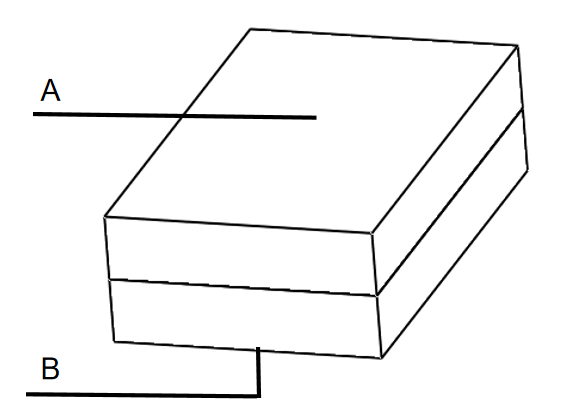
\includegraphics[height=4cm]{figure/双压电晶片示意图.png}
    		\caption{双压电晶片示意图}
    		\label{双压电晶片示意图}
    	\end{minipage}
    \begin{minipage}{0.5\textwidth}
    	\centering
    	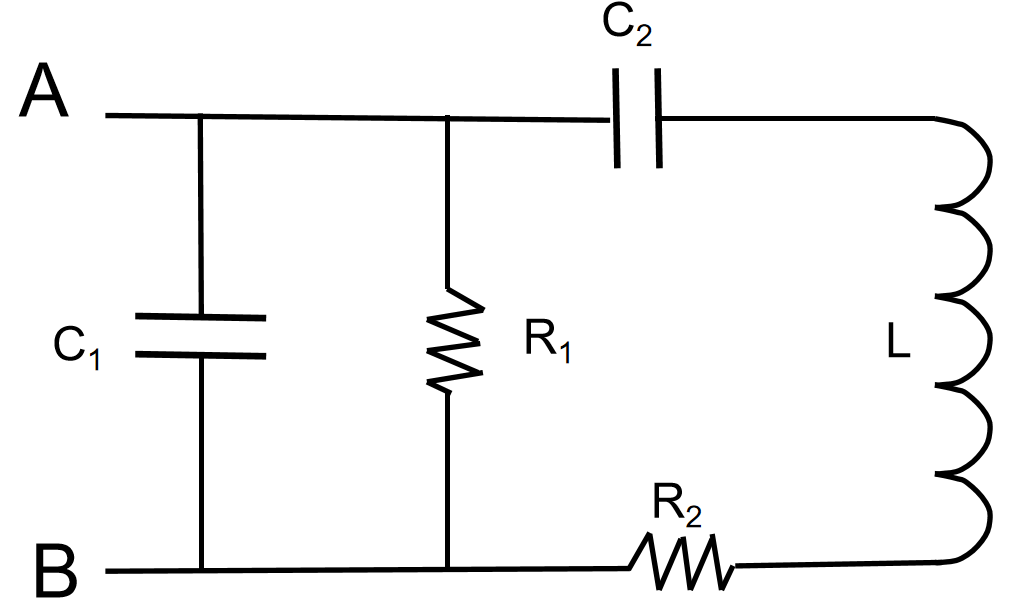
\includegraphics[height=4.25cm]{figure/双压电晶片等效电路.png}
    	\caption{双压电晶片等效电路图}
    	\label{双压电晶片等效电路图}.
    \end{minipage}
    \end{figure}

    双压电晶片如图\ref{双压电晶片示意图}所示,当在AB晶片间施加交流电压时,若片的电场方向与极化方向相同,则起到了增强极化作用的效果,若电场方向与极化方向相反,则对极化作用起到了削弱的效果,利用该原理,可使压电晶片产生与交变电场频率相同的交变形变,当这种形变传递到介质中时,就产生超声波。双压电晶片的等效电路如图\ref{双压电晶片等效电路图}所示。$C_1$为静电电容,$R_1$为陶瓷材料介电损耗并联电阻,$C_2$和$L$为陶瓷材料介电损耗并联电阻,$R_2$为损耗串联电阻\upcite{51单片机超声波测距仪防撞报警倒车雷达设计}。\par

    压电陶瓷晶片有一个固定的谐振频率,即中心频率$f_0$。发射超声波时,施加在其上的脉冲信号频率与固有频率越接近,传感器的分辨率越高。当所用的压电材料不变时,改变压电陶瓷晶片的几何尺寸,就可改变其固有谐振频率。利用这一特性就可制成各种固有频率的超声传感器\upcite{车载可视倒车雷达预警系统的研制16}。
    超声波传感器的结构如图\ref{超声换能器结构图}所示,其主要由金属网、外壳、圆锥形振子、双晶振子、底座和引脚等部分组成 。
    \begin{figure}[!h]
    	\centering
    	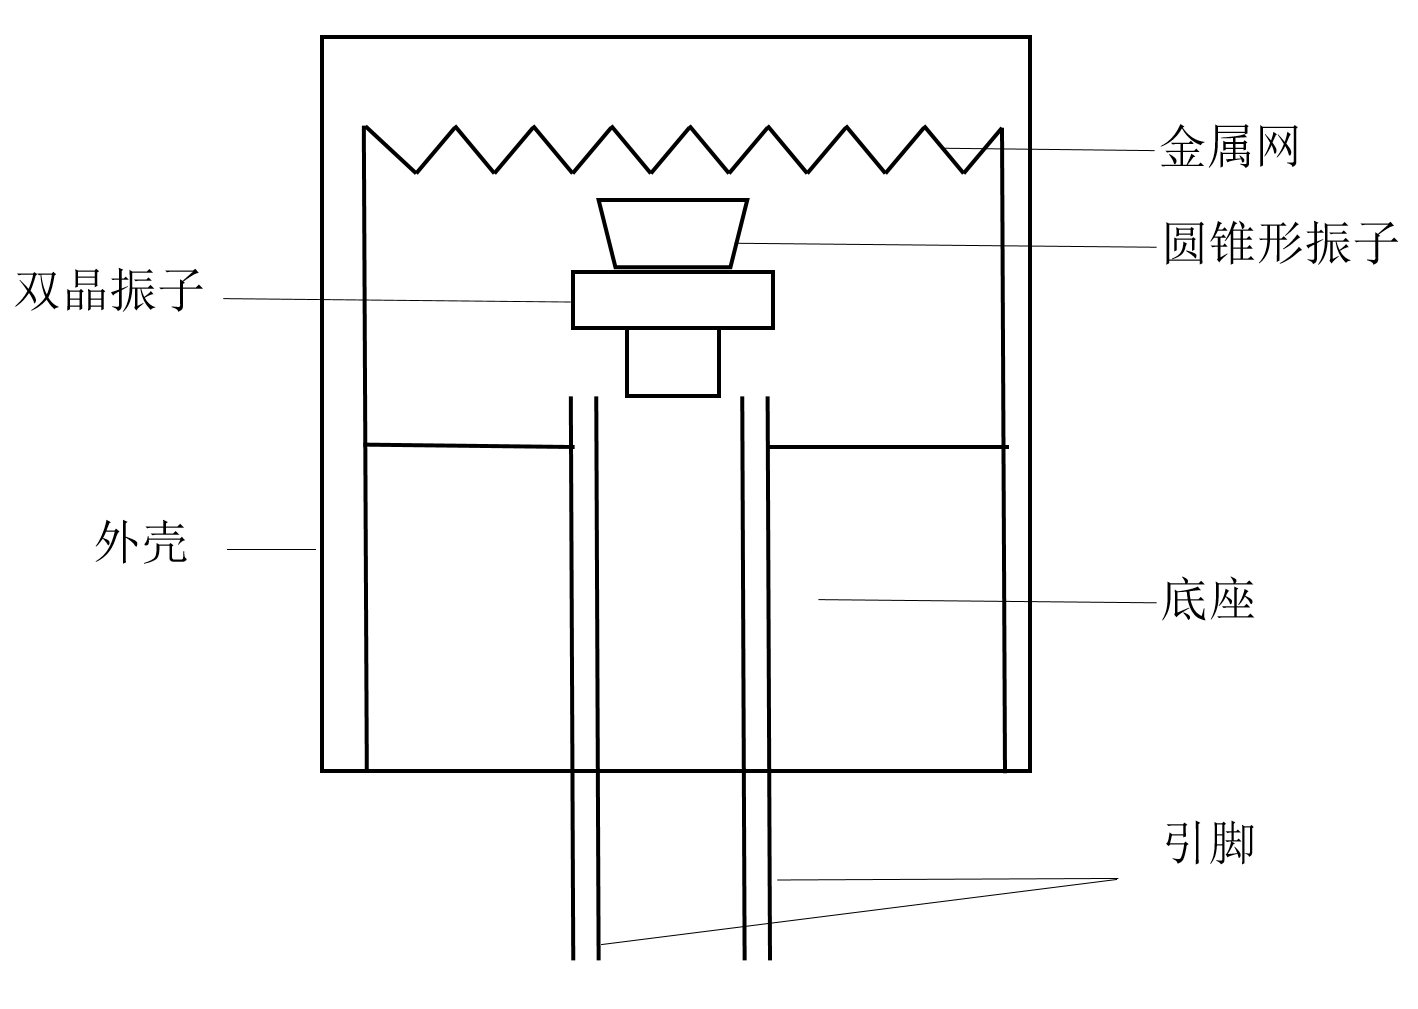
\includegraphics[width=7cm]{figure/超声换能器结构图.png}
    	\caption{超声换能器结构图}
    	\label{超声换能器结构图}
    \end{figure}

    \subsubsection{超声波接近传感器的检测原理}
    \paragraph{连续波相位检测法(CW法))}
    连续波相位检测法的测距原理如图\ref{连续波相位检测法}所示。发射换能器和接收换能器同时发射和接收超声波信号,通过检测信号之间的相位差来获取时间延迟,并计算出传感器与障碍物之间的距离\upcite{面向机器人安全避障的MEMS压电超声接近觉传感器的研究34}。\par
    \begin{figure}[!h]
    	\centering
    	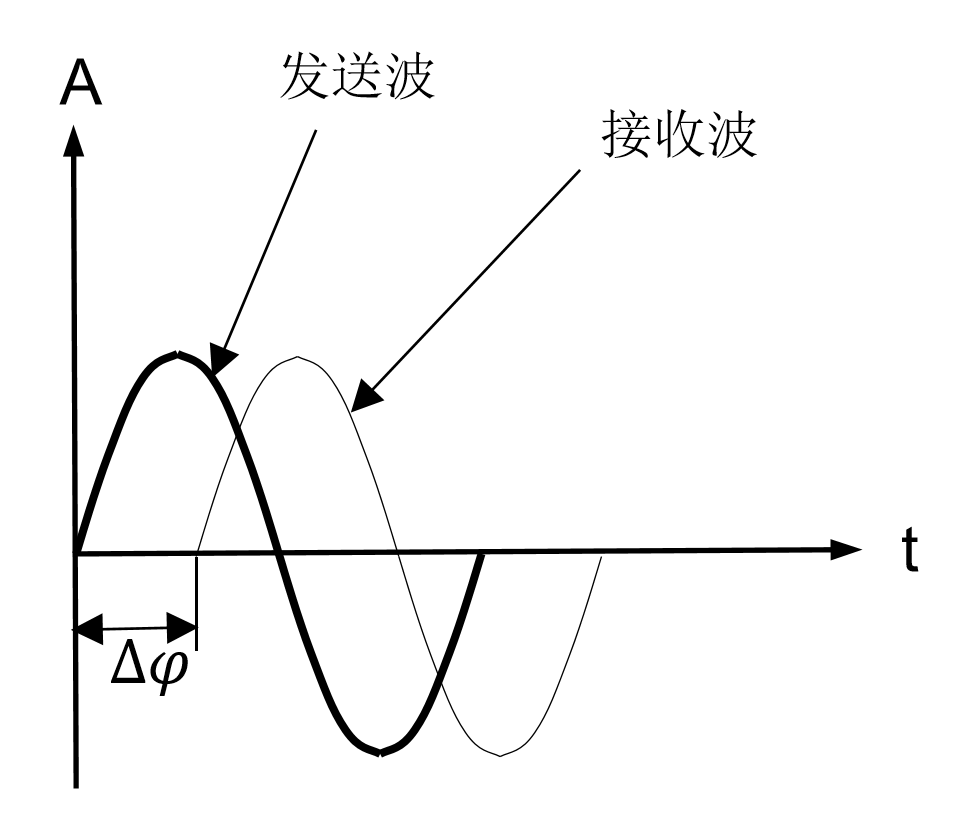
\includegraphics[width=6cm]{figure/连续波相位检测法.png}
    	\caption{连续波相位检测法}
    	\label{连续波相位检测法}
    \end{figure}\par


    假设 发射 的 声 波信 号 为 :
    \begin{equation}
    	u_1=A(x)sin(\omega t + \varphi)
    \end{equation}
式中\quad$\varphi$---初始相位角
接收到的回波信号为:
\begin{equation}
	u_2=A(x)sin(\omega t + \varphi + \omega \cdot{\frac{2D}{c}})
\end{equation}
式中\quad$c$---声速\par
发射声波与回波间的相位差为$\Delta \varphi=\frac{2D}{c}$,传感器与检测物体间的距离D为:
\begin{equation}
	D=\frac{c}{2\omega}\cdot \Delta \varphi=\frac{c}{4\pi f}\cdot(2\pi n + \varphi_i)
\end{equation}
式中\quad$n$---整周期的个数;
\quad$\varphi_i$---不完整周期的相位值。\par
虽然相位检测法的精度比较高,但处理电路的成本也高,需要设计比较复杂的处理电路才能准确地确定回波信号的相位,计算量大\upcite{面向机器人安全避障的MEMS压电超声接近觉传感器的研究35}。\par



    
    \paragraph{飞行时间法}
    飞行时间检测法又称脉冲一回波检测法(如图\ref{飞行时间检测法})。超声换能器发射一组脉冲,在遇到障碍物后脉冲进行反射,换能器在接收到反射回波时,会与发射时刻之间产生时间延迟,该时间延迟称为超声波的飞行时间$t$,飞行时间$t$与声波速度$c$和传播距离$L$有关,即$t=\frac{L}{c}$。
    \begin{figure}[!h]
    	\centering
    	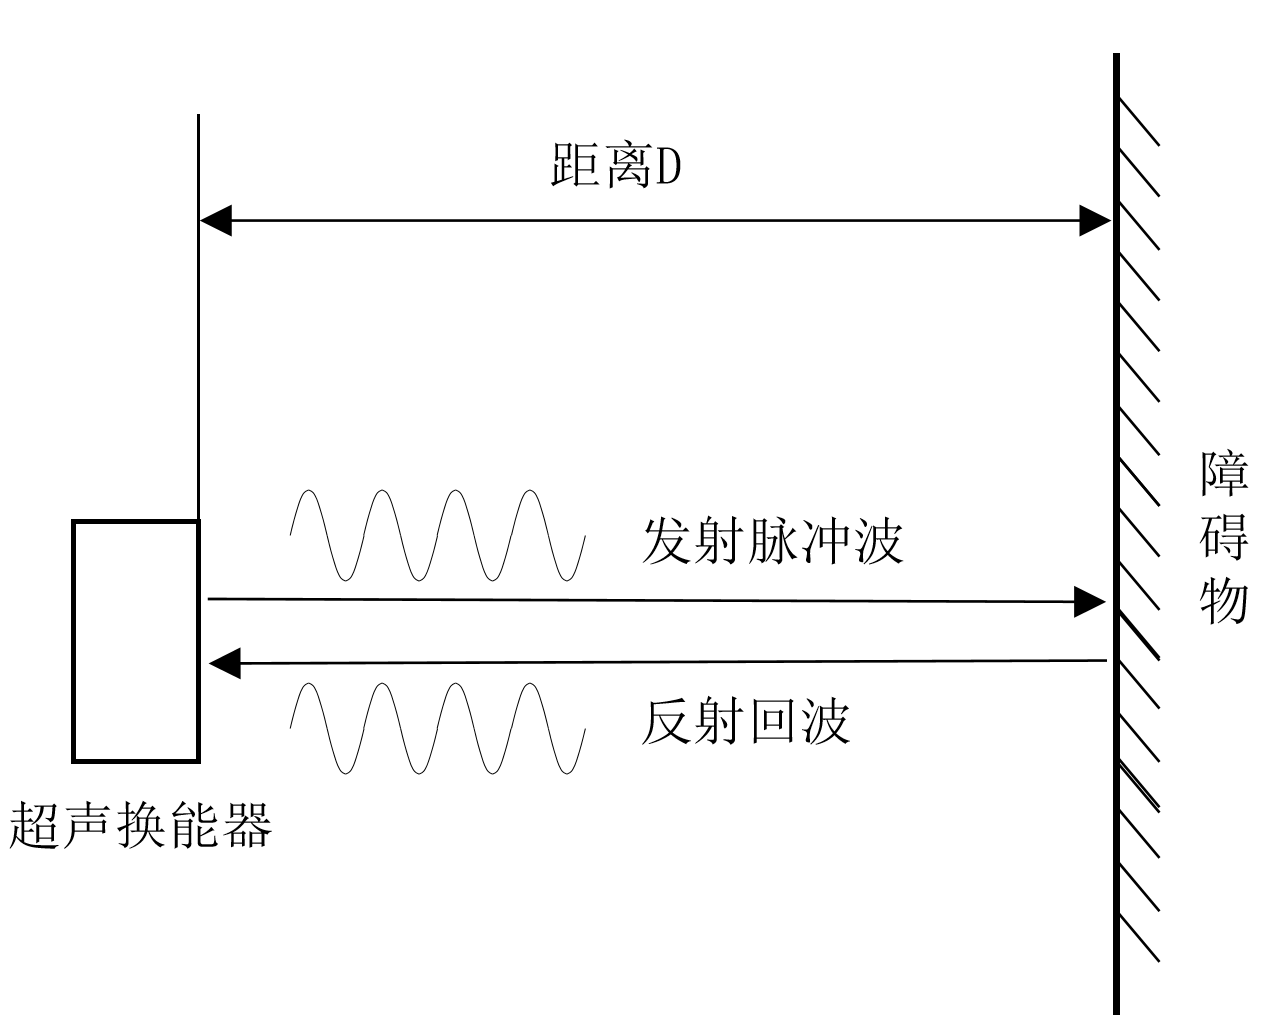
\includegraphics[width=6cm]{figure/飞行时间检测法.png}
    	\caption{飞行时间检测法}
    	\label{飞行时间检测法}
    \end{figure}\par
    飞行时间法最少使用一个换能器便可以实现超声波脉冲的发射和接受,对于自发自收的测距传感器,距离$D$的计算公式为:
    \begin{equation}
    	D=\frac{L}{2}=\frac{ct}{2}
    \end{equation}\par

	采用飞行时间检测法进行障碍物测距,如何简单准确地获得超声波自发射至接收时的飞行时间,是此方法的关键所在。获取飞行时间的方法有很多种,常见的飞行时间法有:互相关函数法、固定阈值法和包络峰值法。\par
	超声波的回波信号相较于发射信号而言,波形基本不变,但在时间上会有一定延迟,因此这两个信号具有相关性。为了准确获取超声波自发射至接收的飞行时间,可以采用相关函数法进行测量。互相关函数法是对超声波的发射信号和回波信号进行互相关函数计算,函数最大值处所对应的时刻就是收发信号相关性最大的时刻,也是回波信号的接收时刻\upcite{面向机器人安全避障的MEMS压电超声接近觉传感器的研究36}。通过计算超声波发射时刻与互相关函数最大值时刻之间的时间差,就可以准确获得超声波的飞行时间。除此之外,固定阈值法和包络峰值法也是常用的飞行时间法。\upcite{面向机器人安全避障的MEMS压电超声接近觉传感器的研究}\par
	固定阈值法是指预先设置一个确定的阈值,当接收的回波信号幅值大于此阈值时,认为此信号幅值所在时刻为回波信号的到达时刻,从而获取超声波的飞行时间。但是在回波信号达到预设阈值时,此时所确定的时刻并不是回波信号的起振时刻,具有一定的时间偏差进行时间补偿将其消除后便可获得飞行时间的估计值。阈值预设大小是固定阈值法用于测量距离的关键因素之一。在固定阈值法中,通过将预设阈值与回波信号的幅值进行比较来判断障碍物距离,而阈值的设置会直接影响到测量结果的精确度。如果阈值设置过高,当障碍物距离较远时,回波信号幅值无法达到阈值大小,导致无法获取飞行时间,从而无法准确测量距离。相反,如果阈值设置过低,噪声信号容易达到阈值大小,造成误触发,导致测量结果不可靠。此外,固定阈值法方法还存在其他问题,例如不同反射距离的回波信号波形幅值大小不同,所造成的时间偏差也不同,简单时间补偿无法获得真实飞行时间,进一步降低了测量结果的精确度。因此,虽然固定阈值法方法简单、易实现、计算量不大,但其精度不高,抗干扰能力差的缺点不能忽视。\par
	包络峰值法是一种常见的获取超声波飞行时间的方法。该方法利用回波信号包络线的峰值所在时刻来获取飞行时间。相比于固定阈值法,该方法更加准确,因为回波信号的幅值会随着传播距离的增加而发生变化,而峰值所在的位置相对回波信号的起振时刻并没有发生变化。此外,回波信号的上升时间与超声波发射信号的频率和周期有关,而与传播距离无关,这种特性也使得包络峰值法可以较好地弥补时间偏差,提高测量精度。值得一提的是,包络峰值法同样存在一些缺点,例如受噪声和杂波的影响较大,需要在实际应用中进行适当的干扰抑制和信号处理。\upcite{面向机器人安全避障的MEMS压电超声接近觉传感器的研究38}。
	       
\subsection{本设计的主要研究内容和论文结构安排}
\subsubsection{主要研究内容}
本设计针对生产线上检测钢化玻璃到位问题,设计了一种稳定性好、灵活性高、应用场景广的超声波接近传感器。
本设计的主要研究内容包括了超声波接近传感器的硬件设计、软件设计和实验设计。\par
硬件设计部分包括了原理图设计和PCB设计,软件设计包括了驱动芯片配置、脉冲信号产生、物体检测三个部分的程序设计以及波形仿真,实验设计部分包括了设计实验进行性能参数测试、稳定性测试和回波特性测试。

\subsubsection{论文结构安排}
本文各章节的主要内容如下:

第二章:提出了超声波接近传感器的总体设计,分为硬件设计、软件设计、实验设计三个部分,初步介绍各个部分的设计流程与方法步骤。然后讲解了在本设计所涉及到的检测原理。

第三章:对传感器的硬件电路设计进行研究,介绍了原理图设计和PCB设计的设计过程。原理图部分的设计分为三部分,分别为:超声波接近传感器控制电路设计、TUSS4470芯片外围电路设计、检测计数电路设计。PCB设计部分主要介绍了TUSS4470外围电路PCB设计,讲解了在PCB设计过程中遵循的几大原则,用于减小各类信号相互之间的干扰,包括了电容、二极管等器件摆放位置优先级,分离接地,铺铜规则等。

第四章:对传感器的软件设计进行研究,首先讲解了传感器所采取的检测策略,然后进行程序的总体设计,根据功能将程序分为了四个模块,分别为:控制模块、SPI模块、脉冲产生模块和检测计数模块。之后分别详细讲解了各个模块的功能、实现原理以及程序流程图。在完成了程序设计方面的工作后,又介绍了如何搭建仿真环境进行程序仿真模拟,最后,给出了仿真模拟后的波形图,并进行了分析。

第五章:设计实验测试传感器的性能以及检测策略的可行性。首先讲解了实物的焊接与调试流程,给出了调试过程中所测得的各引脚波形,然后介绍了实验所用的实验器材,包括虚拟示波器、直尺、各种板材等。最后进行实验,测试了传感器的性能参数、稳定性以及回波特性,给出了实验的结果以及后续分析。

第六章:对本设计存在的不足进行总结,提出了改进的方向,并且进行了对未来的展望。


    \subsection{本章小结}
    本章绪论主要介绍了超声波接近传感器的研究背景和意义,在研究背景中介绍了超声波接近传感器总体的发展情况以及国内外研究现状,然后引出本设计的研究意义是为了设计精度高、稳定性好的传感器。在第二节主要介绍了传感器主要涉及到的原理,包括超声波振幅衰减原理、超声换能器发射脉冲与检测回波信号的原理以及在本设计中的检测原理。在本章的最后一节,则是介绍了本设计的主要研究内容和论文结构安排
    ,并且简单介绍了后几章所包含的内容。
%------------------第三章---------------------------
    \newpage
	\section{超声波接近传感器硬件设计}
	
    \subsection{超声波接近传感器控制电路设计}
    本设计中所使用的CPLD芯片型号为EPM240T100C5N,涉及到的控制电路较简单,在最小系统板的基础上,增加了检测计数电路和TUSS4470外围电路。如图\ref{传感器整体原理图}为传感器整体的原理图,其中主要包括了电源模块、JTAG下载模块、检测计数模块、时钟模块以及复位模块\upcite{CPLD芯片设计指南}。电源
    \begin{figure}[ht]
        \centering
        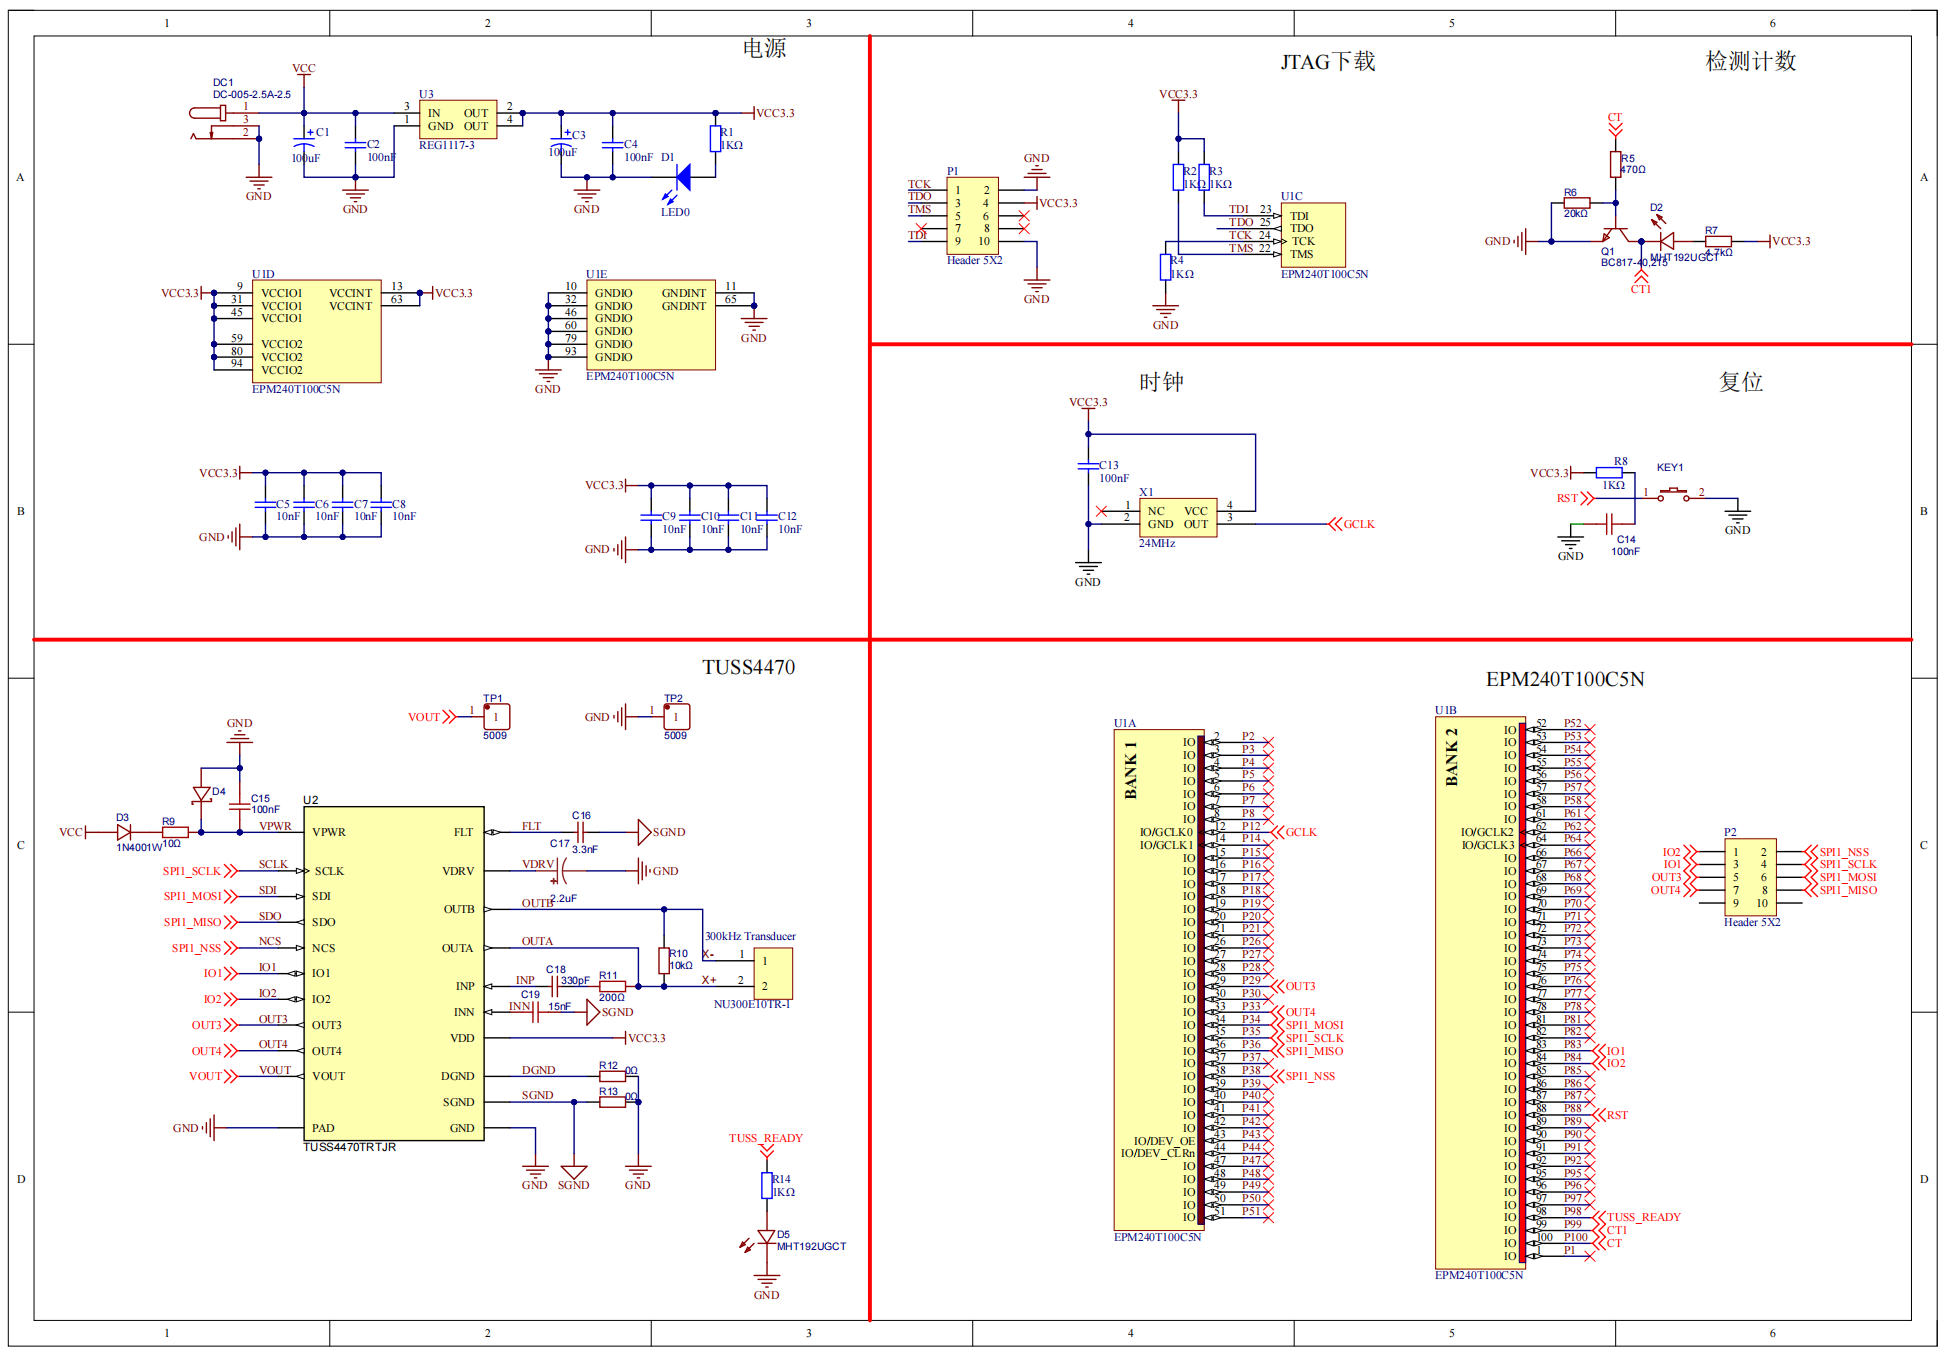
\includegraphics[width=12cm]{figure/Overall circuit.png}
        \caption{传感器整体原理图}
        \label{传感器整体原理图}
    \end{figure}
    \subsubsection{电源模块}
      根据查找芯片手册,可得知EPM240T100C5N的控制电压为:
    TUSS4470芯片的控制电压为3.3V,
    超声探头的驱动电压为:5V-30V\upcite{超声探头手册}。
    可得出电源的设计方案。电源由DC接口、降压芯片、滤波电容组成,可得到12V以及3.3V的电压为各模块供电。电源模块中还包括了一个红色LED指示灯,当模块正常工作时,LED灯就会被点亮。
    
    \subsubsection{JTAG下载模块}
    JTAG(Joint Test Action Group) 下载模块是一种用于编程和调试数字电路和嵌入式系统的通信接口。它通常由三个主要部分组成:JTAG控制器、JTAG下载模块和目标设备。JTAG下载模块的主要作用是将编译后的程序通过JTAG接口下载到目标设备中。在本设计中JTAG主要用于下载烧录调试MCU代码。
    图\ref{JTAG下载模块电路图}左侧为JTAG接头,用于连接下载器,右侧为MCU芯片的连接图其中TCK引脚为测试时钟,
    TDI引脚为测试数据输入,
TDO引脚为测试数据输出,
TMS为测试模式选择,
因为只有一条数据线,通信协议有必要像其他串行设备接口,如SPI一样为串列传输。时钟由TCK引脚输入。配置是通过TMS引脚采用状态机的形式一次操作一位来实现的。每一位数据在每个TCK时钟脉冲下分别由TDI和TDO引脚传入或传出。可以通过加载不同的命令模式来读取芯片的标识,对输入引脚采样,驱动(或悬空)输出引脚,操控芯片功能,或者旁路(将TDI与TDO连通以在逻辑上短接多个芯片的链路)。
    \begin{figure}[ht]
        \centering
        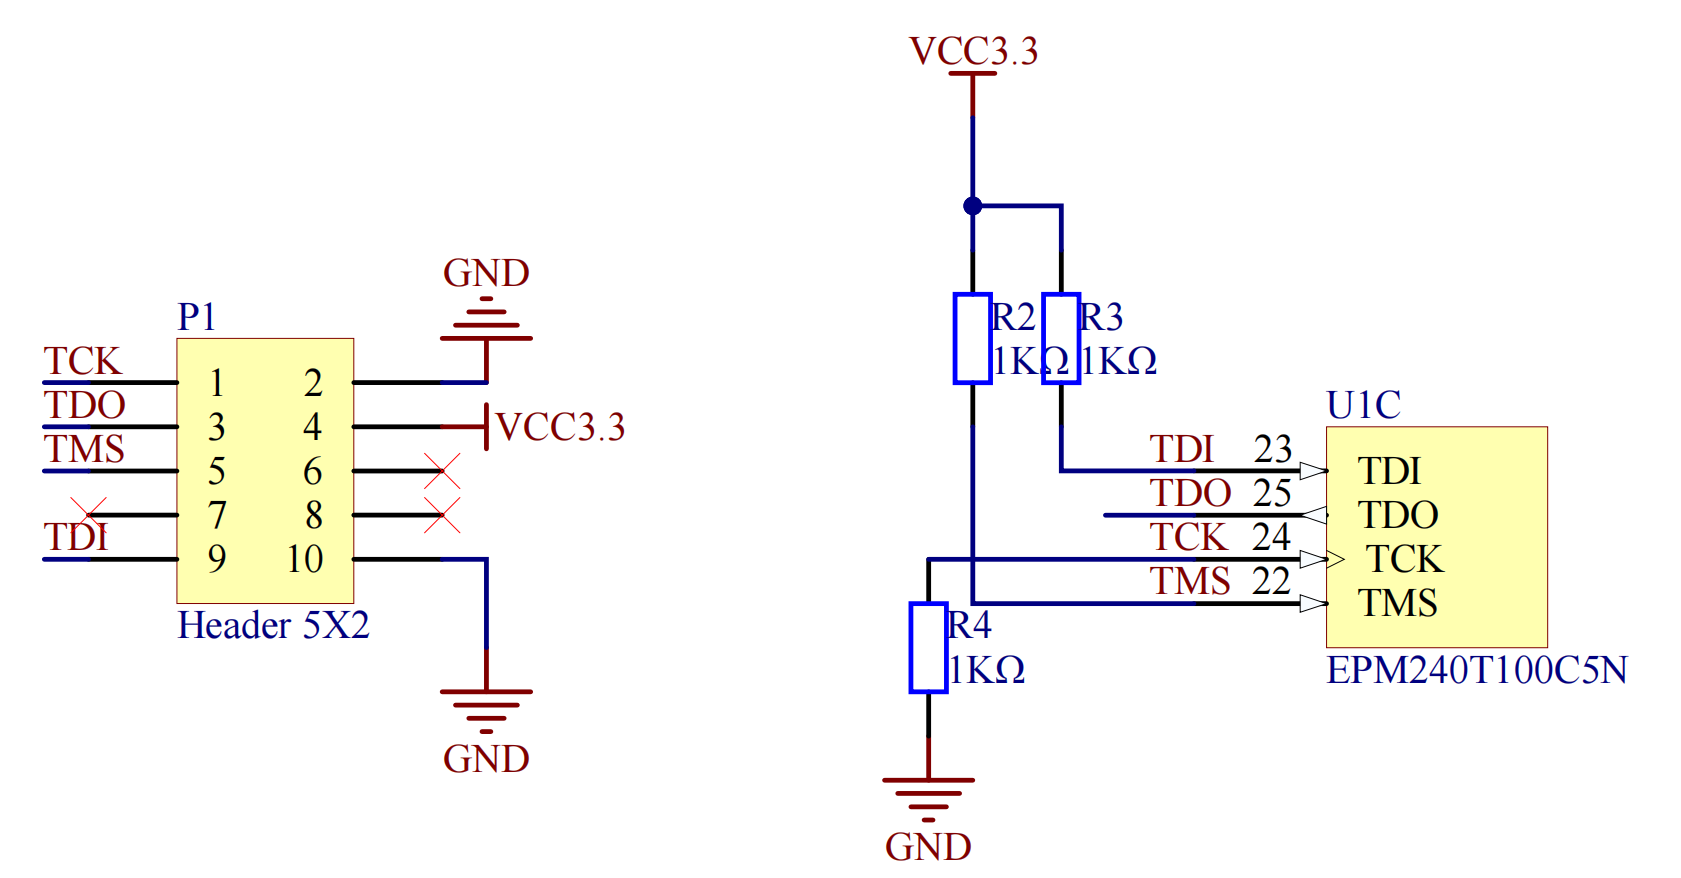
\includegraphics[width=7cm]{figure/JTAG download circuit.png}
        \caption{JTAG下载模块电路图}
        \label{JTAG下载模块电路图}
    \end{figure}
    
    \subsubsection{检测计数模块}
    检测计数模块的功能在于,亮灯提示钢化玻璃到位,并对经过的玻璃进行计数。如图\ref{检测计数模块电路图},CT引脚为MCU输出信号,当程序确定检测到物体后,CT引脚电压拉高,LED灯亮,当物体离开检测范围后,LED等灯灭。CT1引脚则是作为MCU的输入信号,当检测到一次物体后,CT1发出一次脉冲信号,计数加一,以此来实现计数功能。
    \begin{figure}[ht]
        \centering
        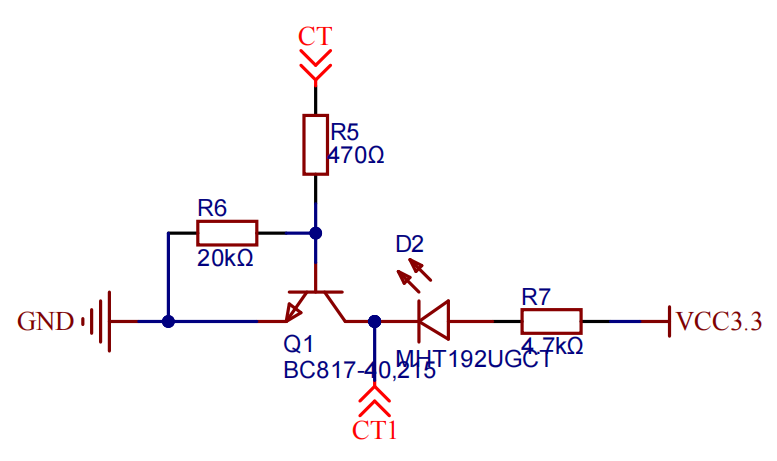
\includegraphics[width=7cm]{figure/detection count circuit.png}
        \caption{检测计数模块电路图}
        \label{检测计数模块电路图}
    \end{figure}
\newpage
       \subsubsection{超声波接近传感器控制电路PCB设计}
       在完成控制电路原理图的设计后,就将进行PCB部分的设计。如图\ref{超声波接近传感器整体PCB设计}为传感器PCB整体设计图,图\ref{超声波接近传感器控制电路PCB设计}为控制电路PCB的设计。
\begin{figure}[ht]
	\centering
	\subfloat[超声波接近传感器整体PCB设计]{
		\begin{minipage}[b]{0.5\textwidth}
			\centering
			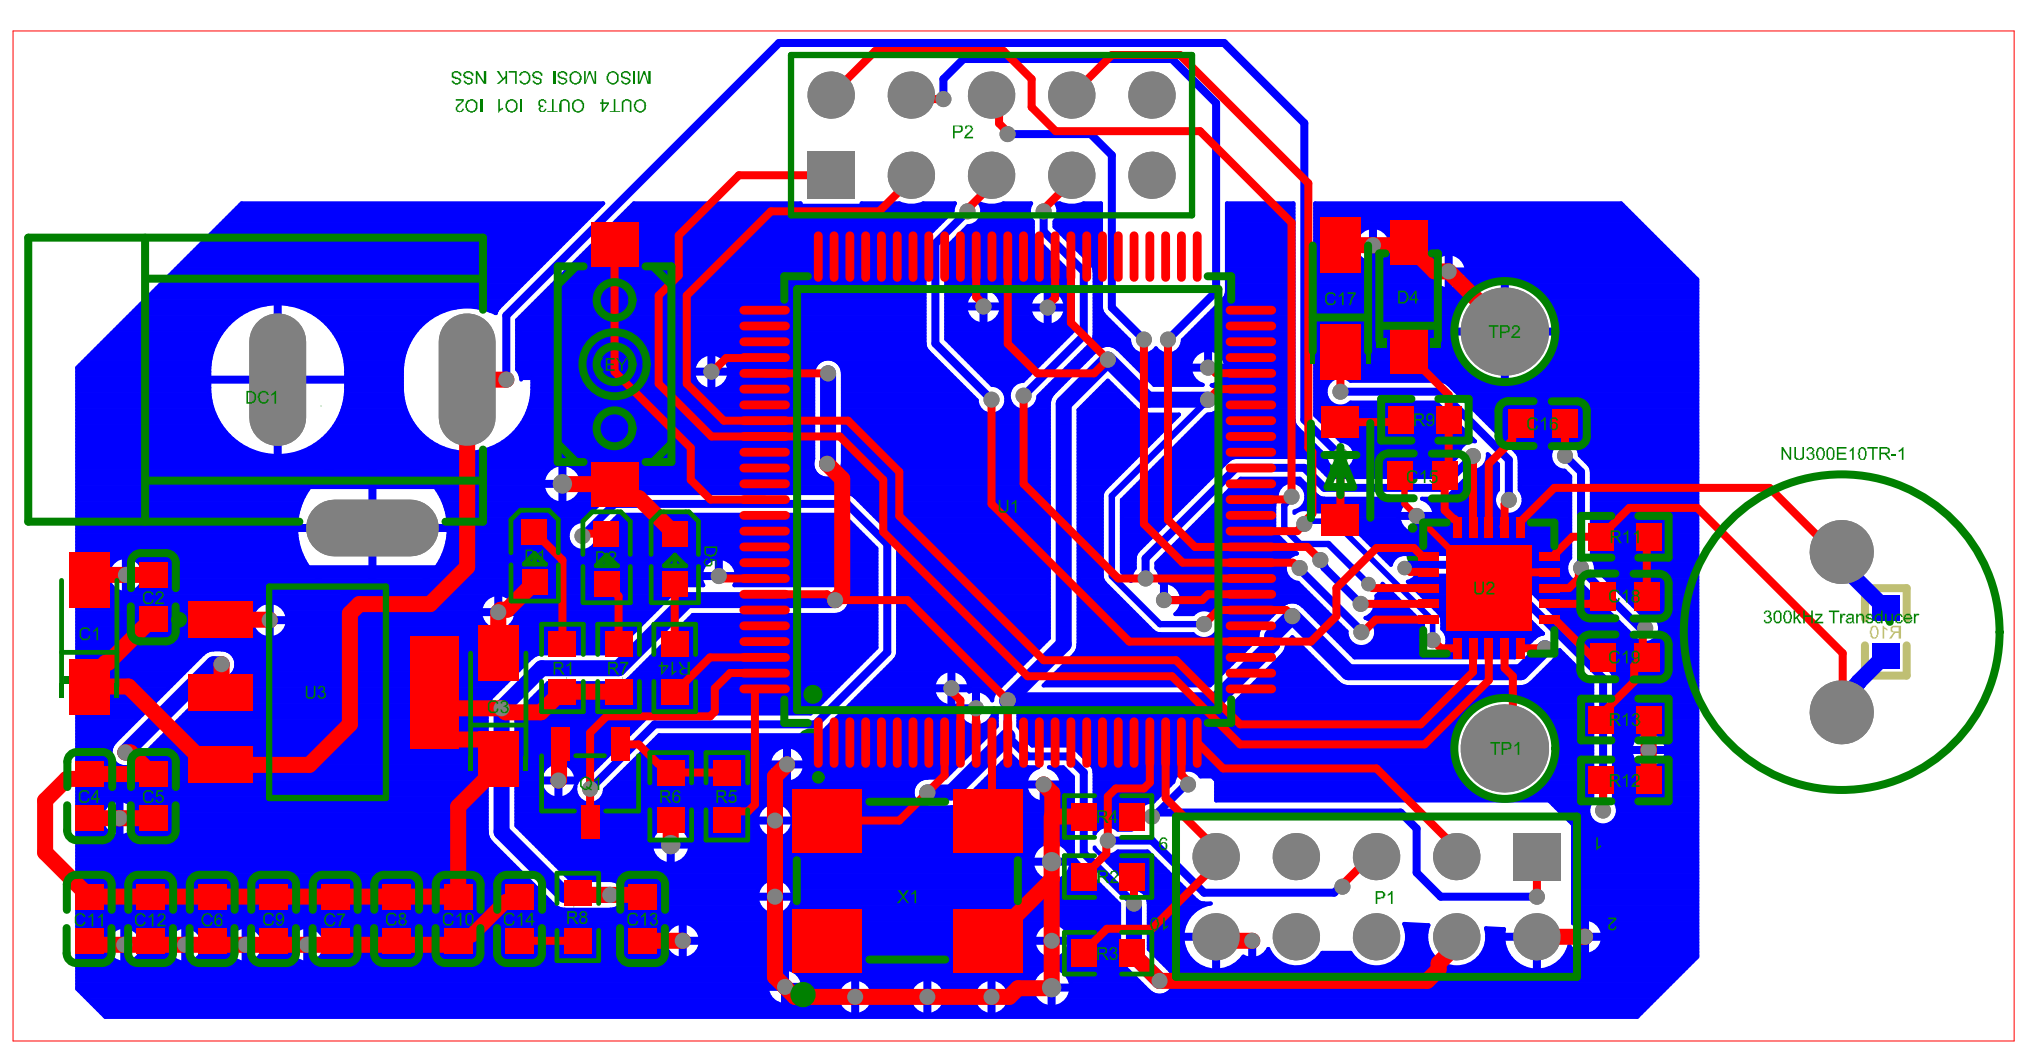
\includegraphics[height=4.5cm]{figure/overall pcb.png}
		\end{minipage}
		\label{超声波接近传感器整体PCB设计}
	}
	\subfloat[超声波接近传感器控制电路PCB设计]{
		\begin{minipage}[b]{0.5\textwidth}
			\centering
			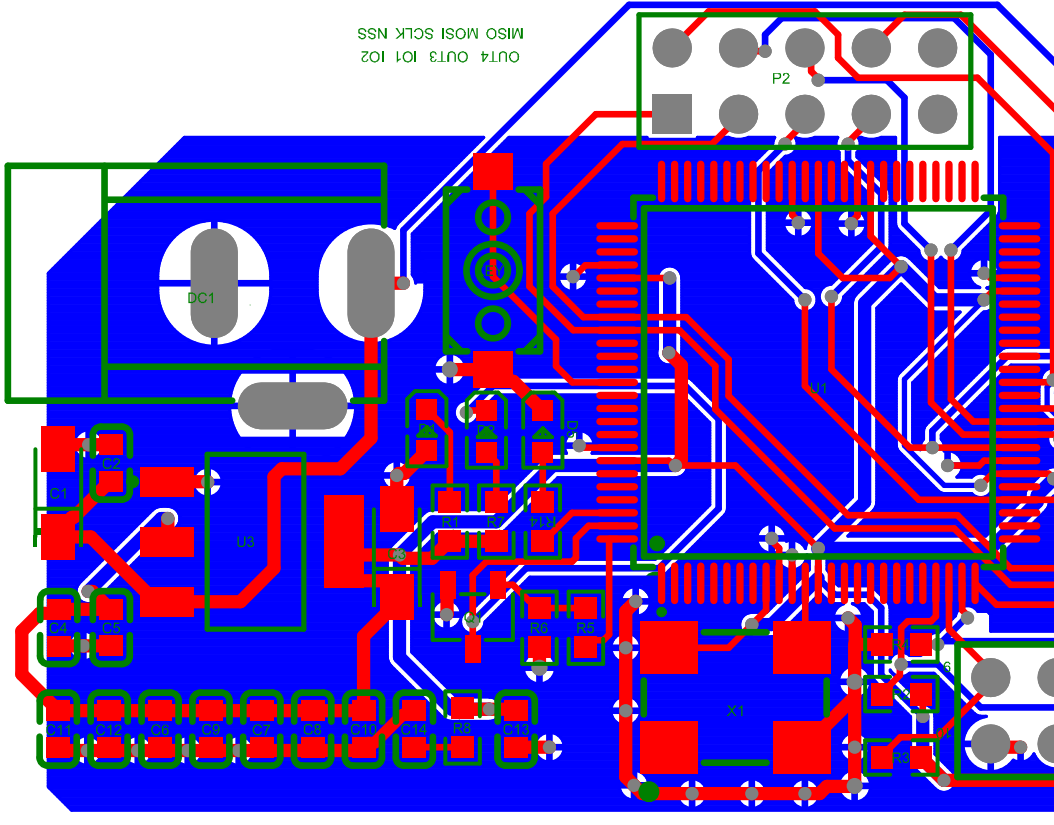
\includegraphics[height=4.5cm]{figure/cpld pcb.png}
		\end{minipage}
		\label{超声波接近传感器控制电路PCB设计}
	}
	\caption{超声波接近传感器PCB设计}
	\label{超声波接近传感器PCB设计}
\end{figure}
   \paragraph{线宽}
   对于功率较大的部分如电源、超声换能器驱动部分,需要对布线进行加宽处理,避免因发热而影响电路板正常工作,甚至产生损坏。\par
   \paragraph{时钟包地处理}
   对于速率较低的时钟,需进行包地处理。包地的作用主要有两点:一是拉开与其他信号的距离,从而减小干扰;二作为自身参考和屏蔽。包地处理还需要在地线上等间距打过孔。
  
 	\newpage
    \subsection{TUSS4470芯片外围电路}
    
    
    \begin{figure}[ht]
		\centering
		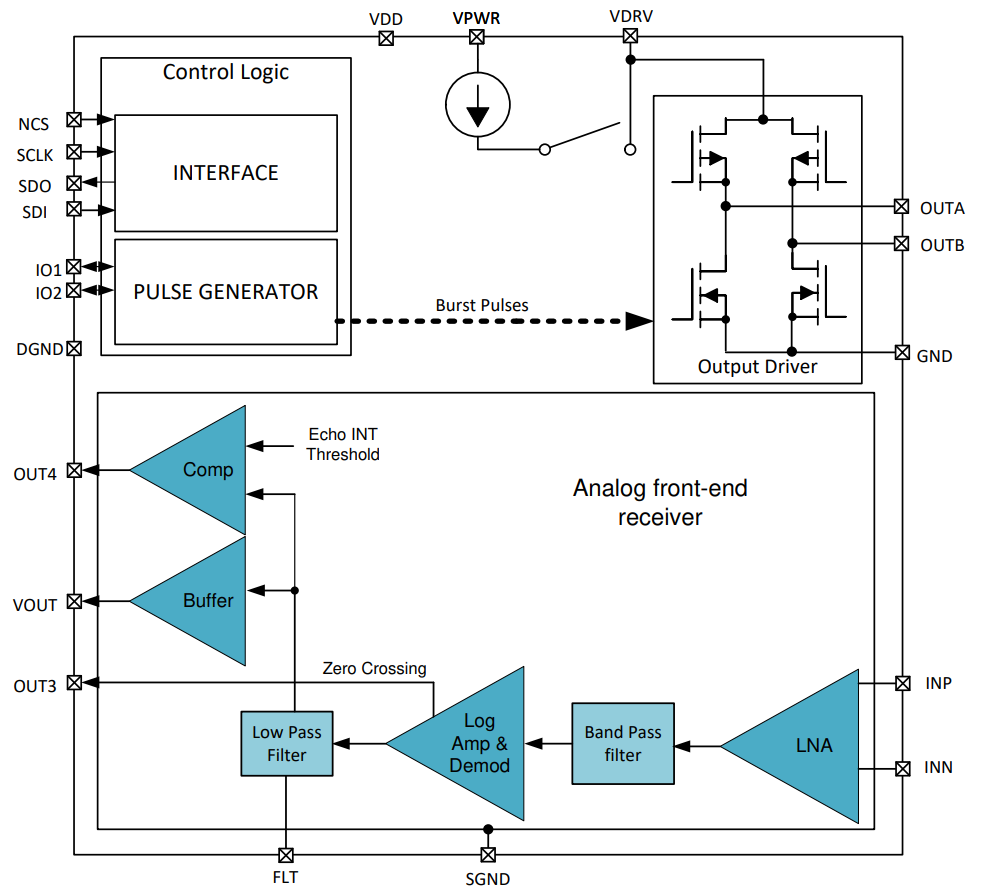
\includegraphics[width=12cm]{figure/Function Block Diagram.png}
		\caption{TUSS4470芯片功能框图}
		\label{TUSS4470芯片功能框图}%文中引用该图片代号
\end{figure}
 图\ref{TUSS4470芯片功能框图}为TUSS4470驱动芯片的整体功能框图\upcite{TUSS4470芯片手册},以此作为外围电路设计的参考资料。如图所示,芯片按照功能可分为逻辑控制、输出驱动、回波接收三个部分。其中逻辑控制部分又分为SPI通信和脉冲发生模块,SPI通信模块用于接收MCU芯片发送的芯片配置数据,脉冲发生模块的两个引脚IO1、IO2连接MCU芯片作为脉冲发生控制引脚,根据芯片不同的IO模式,两个引脚配合产生指定脉宽、脉冲数的脉冲信号;输出驱动模块的OUTA、OUTB引脚直接连接超声换能器,VDRV引脚连接外部电容,VPWR可对电容充电,在VDRV到达设定电压值后,VPWR停止对VDRV供电,这使得超声换能器的驱动电压可以保持在设定值,以此保证发出脉冲的声压水平可以稳定在一定水平,从而保证发射出稳定的脉冲波(其中VDRV的设定电压可通过SPI对芯片进行配置);回波接收模块的作用在于:对回波信号进行处理,输出可供MCU进行检测判断的信号其中INP、INN引脚连接超声波换能器的正负端,FLT连接外部电容作为低通滤波器对回波信号进行滤波处理。OUT3引脚内部连接至模块中的对数解调模块,当回波信号在模块内进完成放大进行解调时,将某阶段信号作为零点,输出过零信号,以验证接收信号的频率, 提高对其他信号的抗干扰性。OUT4作为检测到位的指示信号,当VOUT输出电压超过芯片配置数据中设定的阈值时,OUT4拉高。(VOUT引脚的电压值由公式\ref{VOUT公式}决定)。
  
    \begin{equation}
        V_{OUT}=G_{VOUT} \cdot SL_{LOG}\cdot20log_{10}(\frac{G_{LNA} \cdot G_{BPF} \cdot V_{IN}}{INT_{LOG} \cdot K_X})
        \label{VOUT公式}
    \end{equation}
式中\quad $G_{VOUT}$---对数放大器斜率增益调整(Slope or gain adjustment);\par
\quad$SL_{LOG}$---对数运算放大器斜率调整(slope of logarithmicamplifier);\par
\quad$G_{LNA}$---回波增益;\par
\quad$G_{BPF}$---$0.9v/v$;\par
\quad$V_{IN}$---INN引脚输入;\par
\quad$INT_{LOG}$---对数放大器截距( logarithmic amplifier intercept);\par
\quad$K_X$---对数截距平差(log intercept adjustment)\par
    回波接收模块的详细工作框图如图\ref{回波接收模块}所示。
    \begin{figure}[ht]
        \centering
        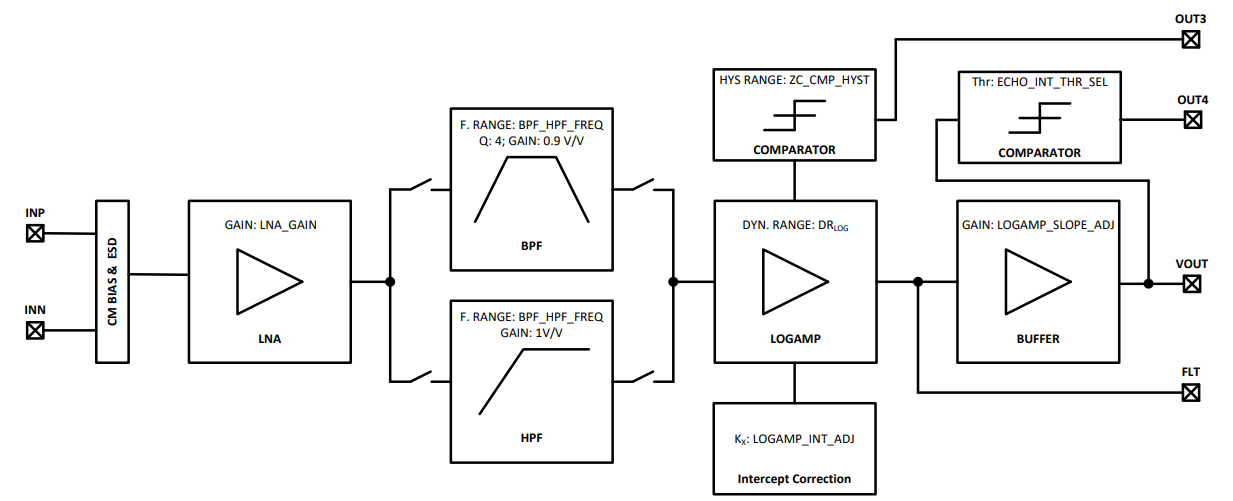
\includegraphics[width=10cm]{figure/Analog Front-End Block Diagram.png}
        \caption{回波接收模块}
        \label{回波接收模块}
    \end{figure}\par

    参考芯片手册相关内容,进行了TUSS4470芯片外围电路的设计,如图\ref{TUSS4470芯片外围电路}所示。
    \begin{figure}[!h]
        \centering
        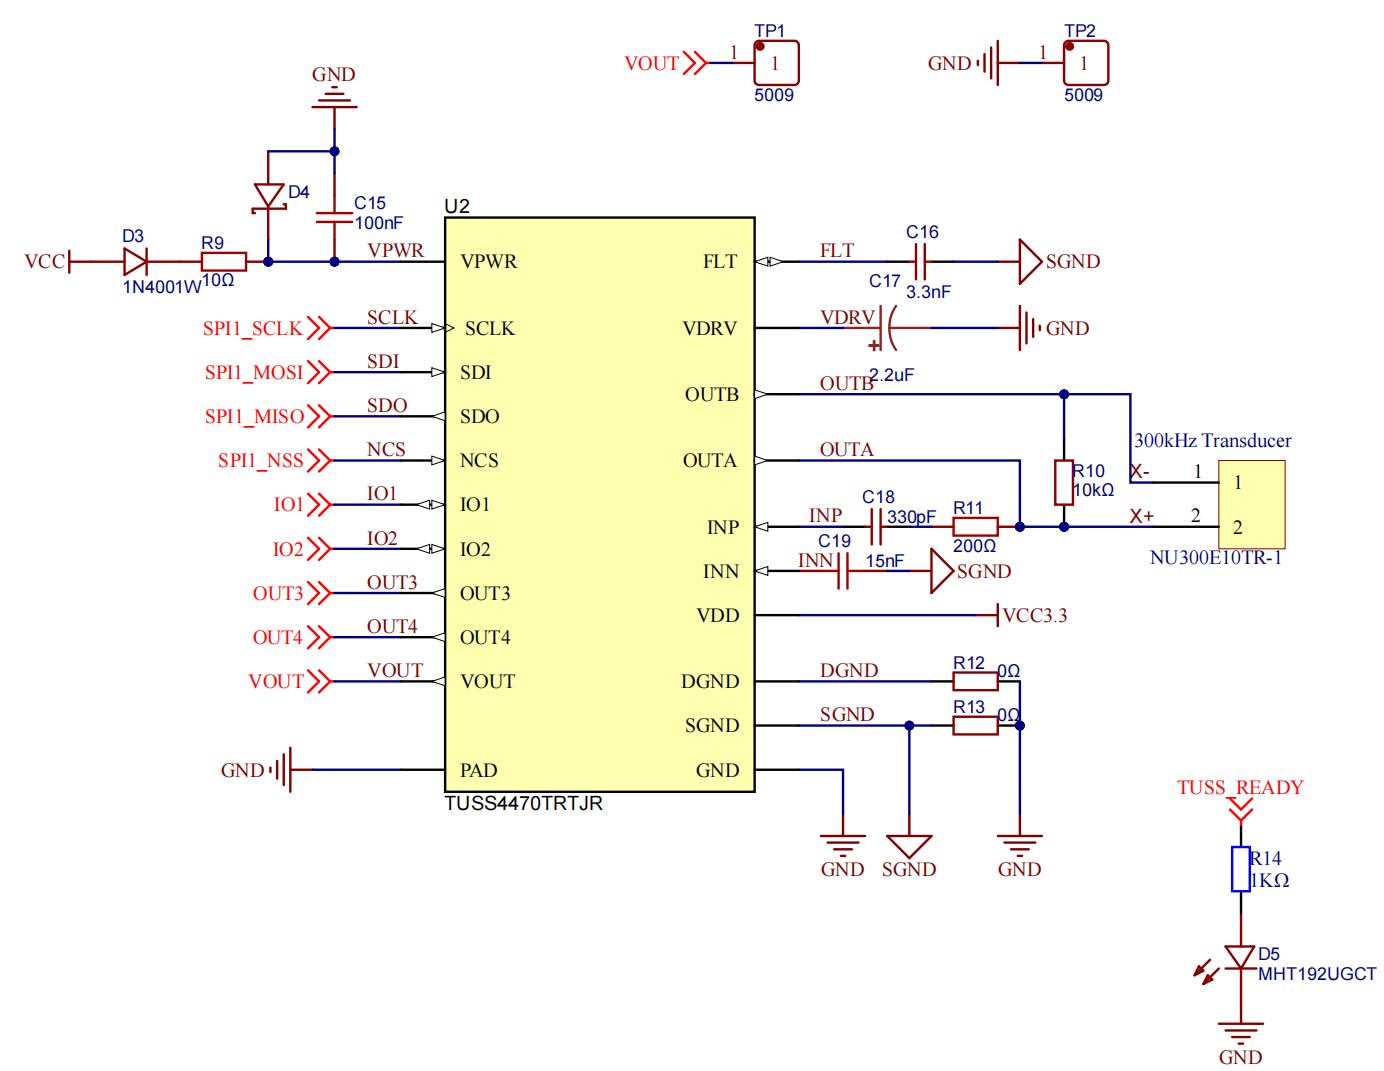
\includegraphics[width=9cm]{figure/TUSS4470 peripheral circuit.png}
        \caption{TUSS4470芯片外围电路}
        \label{TUSS4470芯片外围电路}
    \end{figure}
\newpage
    \subsubsection{VPWR引脚电路}
    VPWR引脚输入电压范围为5V到36V,TUSS4470设备可能受到电池瞬变和反向电流的影响,因此采用外部组件保护芯片十分必要。图\ref{VPWR引脚}中除了靠近引脚的电容C15,二极管D3、D4和电阻R9就起到了保护芯片的作用。
     \begin{figure}[ht]
    	\centering
    	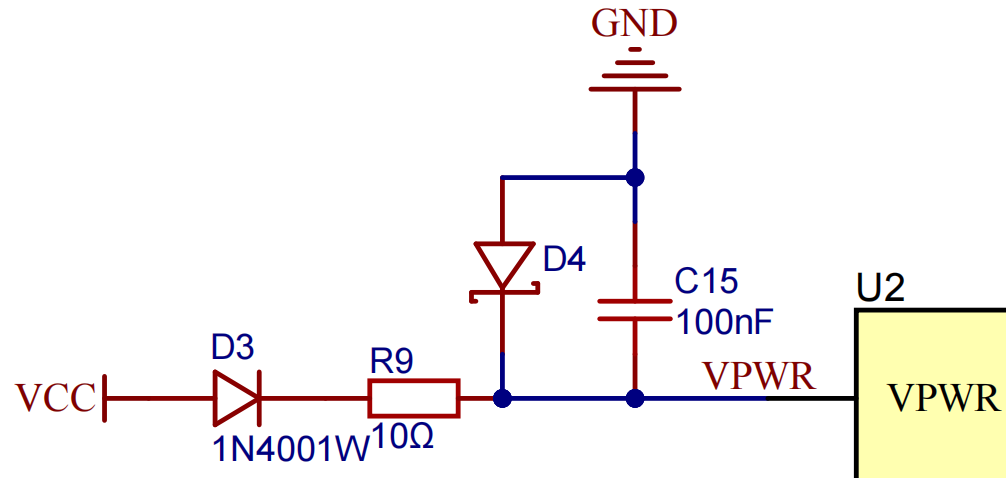
\includegraphics[width=10cm]{figure/VPWR PIN.png}
    	\caption{VPWR引脚电路}
    	\label{VPWR引脚}
    \end{figure}
        \subsubsection{FLT外接滤波电容}
    FLT引脚外接滤波电容,对应图\ref{TUSS4470芯片功能框图}回波检测模块中的低通滤波器。该滤波电容的作用在于,去除对数放大器输出中的高频信号,使解调包络信号有足够的峰值保持时间,而截止频率的大小则由FLT引脚的阻抗以及外接电容的电容量所决定,该电容虽然可以抑制高频信号的波动,但同样会减缓信号的响应速度。大电容量可以使VOUT引脚输出的电压峰值变化减小,并且减缓上升下降到峰值的时间,而最优电容量则需在应用中不断进行优化。本设计初步使用电容量为3.3nF的电容。
    \subsubsection{VDRV引脚电路}    
    VDRV引脚连接外部电容,TUSS4470芯片通过VPWR引脚为外部的电容充电,当其达到设定电压时则停止充电,此时该电容将为超声换能器H桥驱动电路供能。
     \subsubsection{超声换能器驱动电路}
    在TUSS4470的芯片手册中,超声换能器有四种不同的驱动方式,不同驱动方式产生脉冲的方式也不同,本设计中采用最典型的HALF\_BRG\_MODE\_0来进行驱动,如图\ref{参考配置方式}为参考配置方式,图\ref{实际配置方式}为本设计中所采用的方式。
    
\begin{figure}[ht]
	\centering
	\subfloat[参考配置方式]{
		\begin{minipage}[b]{0.5\textwidth}
			\centering
			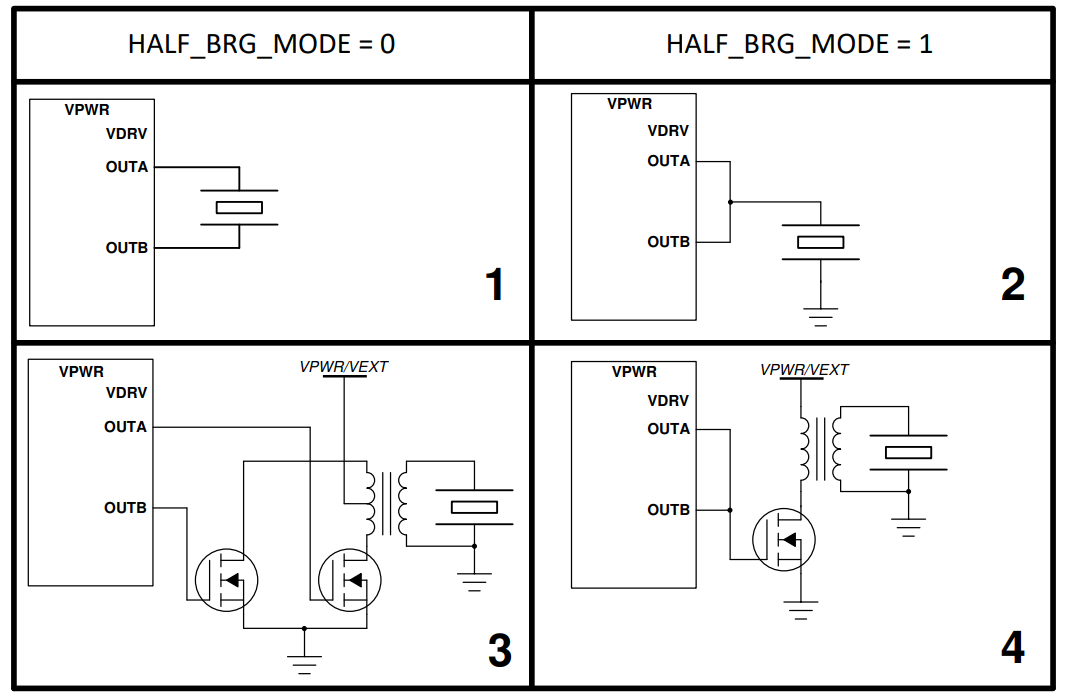
\includegraphics[height=4.5cm]{figure/TUSS4470 Transducer Drive Options.png}
		\end{minipage}
		\label{参考配置方式}
	}
	\subfloat[实际配置方式]{
		\begin{minipage}[b]{0.5\textwidth}
			\centering
			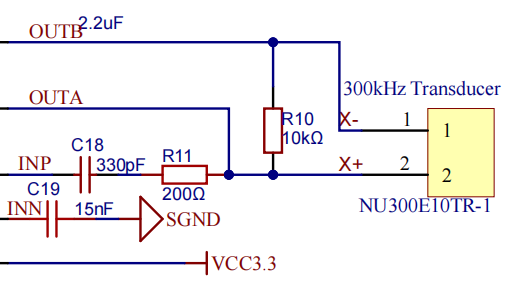
\includegraphics[height=4.5cm]{figure/OUTA PIN.png}
		\end{minipage}
		\label{实际配置方式}
	}
	\caption{超声换能器驱动电路设计}
	\label{超声换能器驱动电路设计}
\end{figure}
    \subsubsection{芯片配置指示电路}
    CPLD芯片通过SPI协议向TUSS4470芯片发送配置数据,并接收其反馈回数据。在芯片返回的数据当中,有一位的状态位用来反映芯片是否准备就绪,当芯片准备就绪后该位置1,可供MCU进行下一步的工作。如图为芯片配置指示电路,当芯片配置就绪后,MCU该引脚拉高,LED灯亮,用来指示芯片的配置状态。
    \subsubsection{分离接地电路}
    由于外围电路中包含多种类型的信号,例如VPWR引脚的电源信号,VOUT引脚的模拟信号,VOUT引脚的模拟信号,SCLK等引脚的数字信号。当产生数字信号的引脚产生脉冲时,其变换速度较快,将会在数字地产生较大的噪声;而模拟信号又容易受到外接的干扰,如果将数字信号和模拟信号直接接入同一个大地,将会严重影响模拟信号的准确性,对于超声波传感器而言,是非常致命的。本设计在原理图设计的过程中便解决了不同类型分离接地\upcite{分离接地}的问题,采用的方法是:先将不同类型的信号连接到0$\Omega$电阻,再连接到大地,0$\Omega$电阻相当于很窄的电容通道,能够有效的限制环路电流,使噪声得到抑制。起分离接地作用的电路如\ref{分离接地电路}所示。
     \begin{figure}[!h]
        \centering
        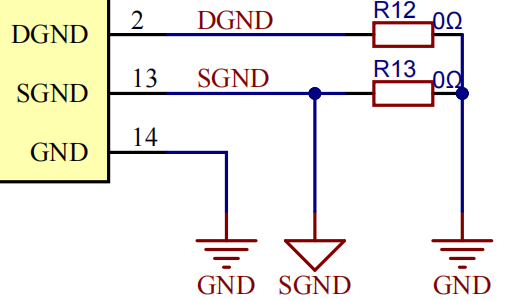
\includegraphics[width=7cm]{figure/seperate ground.png}
        \caption{分离接地电路}
        \label{分离接地电路}
    \end{figure}
	\subsubsection{TUSS4479芯片外围电路PCB设计}
    由于本设计中涉及到的信号类型较多,包括了数字信号、模拟信号、高频信号、大功率信号,各信号间会存在较大的干扰,因此在布线过程中将各信号分离十分重要,直接关系到传感器的稳定性和精度。如图\ref{TUSS4470芯片外围电路PCB设计}为TUSS4470芯片外围电路PCB设计,图\ref{TUSS4470芯片引脚图}为芯片对应的引脚图。本设计采用两层板来完成布线。
  \begin{figure}[!h]
   		\begin{minipage}[t]{0.5\linewidth}
  			\centering
  			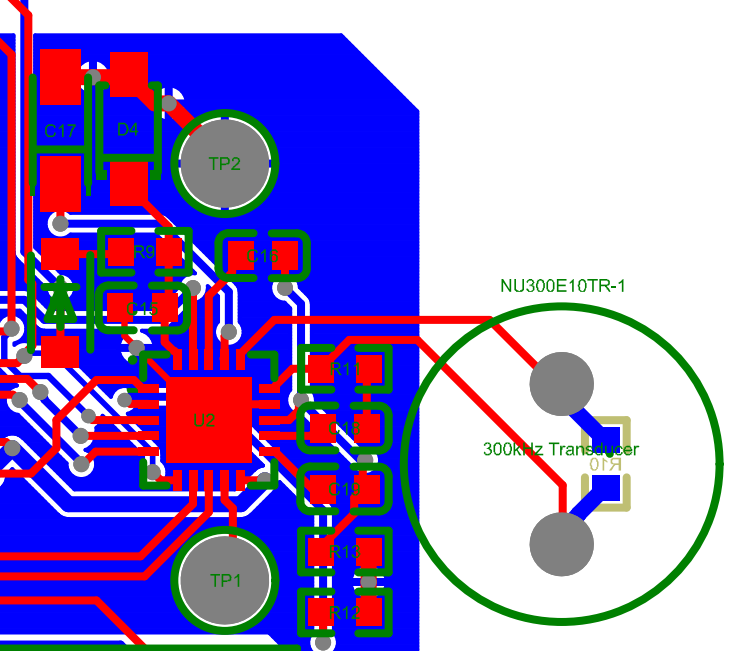
\includegraphics[height=5cm]{figure/TUSS4470 pcb.png}
  			\caption{TUSS4470芯片外围电路PCB设计}
  			\label{TUSS4470芯片外围电路PCB设计}
  		\end{minipage}
   		\begin{minipage}[t]{0.5\linewidth}
  			\centering
  			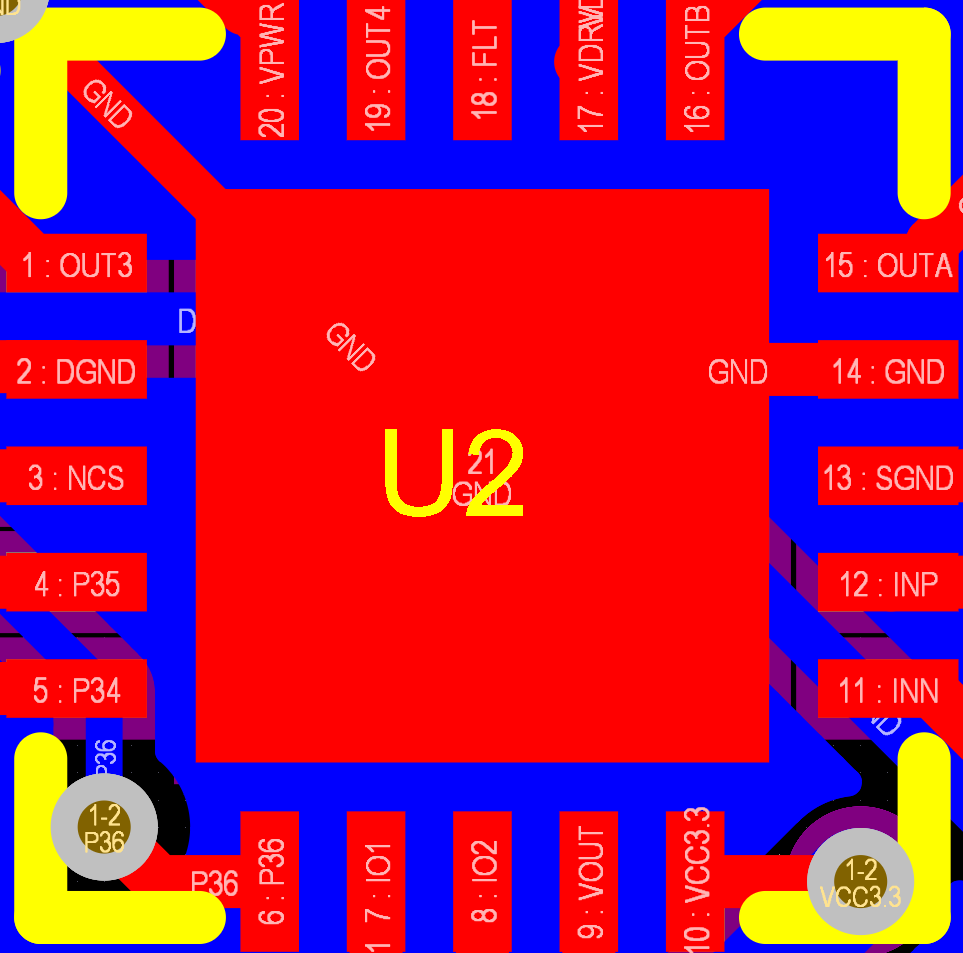
\includegraphics[height=5cm]{figure/TUSS4470 PIN.png}
  			\caption{TUSS4470芯片引脚图}
  			\label{TUSS4470芯片引脚图}
  		\end{minipage}  		 
  \end{figure}\par
    在TUSS4470驱动芯片的PCB设计过程中,最重要的就是将芯片的电源信号、数字信号以及模拟信号进行分离。参考芯片手册\upcite{TUSS4470芯片手册},在布线时考虑到了如下事项。\par
    \paragraph{各类信号分离接地}
    在连接到主地前,数字接地、传感器接地、回波接地都要先通过0$\Omega$电阻或者铜迹线,如图\ref{分离接地电路},本设计在原理图设计时采用了0$\Omega$电阻的方式来实现分离接地,因此在布线时就不需要考虑该问题。
     \paragraph{回波接收引脚}
    INN、INP引脚作为回波信号的接收引脚,对噪声干扰十分敏感,所以其布线必须要短且直,并且保证INN引脚的电容尽量靠近芯片引脚,以减少干扰,但考虑到后续需手工焊接,电容与芯片引脚间仍要保持一定的间隙,以减小手工焊接的难度。假设不考虑测试成本,采用贴片工艺,电容与芯片引脚间的距离还可再进一步减小,以获得到具有更高稳定性的回波信号。
    \paragraph{VOUT引脚}
    VOUT引脚作为模拟信号输出端,与外界的连线应该尽量短直,避免产生寄生效应\upcite{寄生效应},以及外部噪声干扰引起的噪声耦合。\par
    \paragraph{超声换能器驱动}
    芯片与OUTA、OUTB引脚间的布线应尽可能短且直,以保证发出脉冲信号的质量,从而提高传感器的精度。考虑到两个引脚输出的是大功率、高频率的模拟信号,连接到两引脚的线宽应不能太小。\par
    \paragraph{VPWR引脚}
        根据芯片手册推荐,VPWR的解调电容应尽可能靠近引脚。\par
     \paragraph{信号分离}
     数字信号引脚如TXD、RXD、 SCLK、 NCS、IO1、 IO2、 OUT3、OUT4应远离模拟信号引脚,避免信号间的干扰。\par
\subsection{本章小结}
本章主要介绍了超声波接近传感器硬件部分的设计,首先介绍了超声波接近传感器控制电路的设计,该部分包括了原理图设计和PCB设计,重点讲解了JTAG下载模块的设计和时钟包地处理。然后又详细介绍了TUSS4470芯片外围电路的设计,该部分讲解了各管脚连接器件的选型以及PCB设计过程中需要注意的事项,原理图设计部分详细介绍了VPWR引脚、VDRV引脚以及各类信号分离接地处理的设计,而PCB设计部分则详细介绍了各类器件的布局原则,以减少信号间的相互干扰。\par
至此已介绍完成了超声波接近传感器原理图设计和PCB设计部分的工作,下一章将详细讲解传感器的软件设计部分。

      
    
    
    












\end{document}